\documentclass[../Article_Model_Parameters.tex]{subfiles}
\graphicspath{{\subfix{../Figures/}}}
\begin{document}
	
	\subsubsection{Uneven solute's distribution in the solid phase} \label{CH: Gamma_Function}
	
	Following the idea of the Broken-and-Intact Cell (BIC) model (\citet{Sovova2017}), the internal diffusion coefficient $D_i$ is considered to be a product of the reference value of $D_i^R$ and the exponential decay function $\gamma$, as given by Equation \ref{EQ: C_sat_function}:
	
	{\footnotesize
		\begin{equation}
			D_i = D_i^R \gamma(c_s) = D_i^R \exp \left( \Upsilon \left( 1-\cfrac{ c_s }{c_{s0}} \right) \right) \label{EQ: C_sat_function}
	\end{equation} }
	
	where  ${\color{black}\Upsilon}$ describes the curvature of the decay function. Equation \ref{Model_kinetic} describes the final form of the kinetic term:
	
	{\footnotesize
		\begin{equation}
			\label{Model_kinetic}
			r_e = -\cfrac{D_i^R \gamma }{ \mu l^2 } \left( c_s  - \cfrac{\rho_s c_f }{ k_m \rho_f }  \right)
	\end{equation} }
	
	The $\gamma$ function limits the solute's availability in the solid phase. Similarly to the BIC model, the solute is assumed to be contained in the cells, some of which are open because the cell walls were broken by grinding, with the rest remaining intact. The diffusion of the solute from a particle's core takes more time than the diffusion of the solute close to the outer surface. The same idea can be represented by the decaying internal diffusion coefficient, where the decreasing term is a function of the solute concentration in the solid. 
	
	An alternative interpretation of the decay function $\gamma$ involves considering the porous structure of the solid particles, where the pores are initially saturated with the solute. During extraction, the solute within these pores gradually dissolves into the surrounding fluid. Initially, the solute molecules near the pore openings dissolve and diffuse rapidly due to the short diffusion paths. As the extraction progresses, the dissolution front moves deeper into the pore structure, and solute from the inner regions of the pores begins to dissolve. The diffusion of solute molecules from the interior of the pores to the external fluid becomes progressively slower because the effective diffusion path length increases. This lengthening of the diffusion path enhances the mass transfer resistance, reducing the overall diffusion rate. 
		
	In an extreme case, this model could be compared with the Shrinking Core Model presented by \citet{Goto1996}, where the particle radius decreases as the solute content in the solid phase diminishes. In the SC model, the reduction in particle size leads to significant changes in both the diffusion path length and the surface area available for mass transfer. The diminishing particle size increases the diffusion path within the remaining solid core and decreases the external surface area, both of which contribute to a slower extraction rate. By comparing this to the varying diffusion coefficient in our model, some conceptual similarities can be noticed.
	
	\subsubsection{Empirical correlations}
	
	The empirical correlations for $D_i$ and $\Upsilon$ were derived by \citet{Sliczniuk2024} and validated for temperatures between $30 - 40~^\circ C$, pressures between $100 - 200$ bar, and mass flow rates between $3.33-6.67 \cdot 10^{-5}$ kg/s. Figures \ref{fig:Correlation_Di} and \ref{fig:Correlation_Gamma} show the results of multiple linear regression applied to solutions of parameter estimation and selected independent variables. The region marked with the white dashed line represents the confidence region, where the model has been tested. Both correlations should be equal of greater than zero, to avoid unphysical behaviour such as the reverse mass transfer. The multiple linear regression functions are combined with the rectifier function to ensure the non-negativity.
	
	\begin{figure}[!ht]
		\centering
		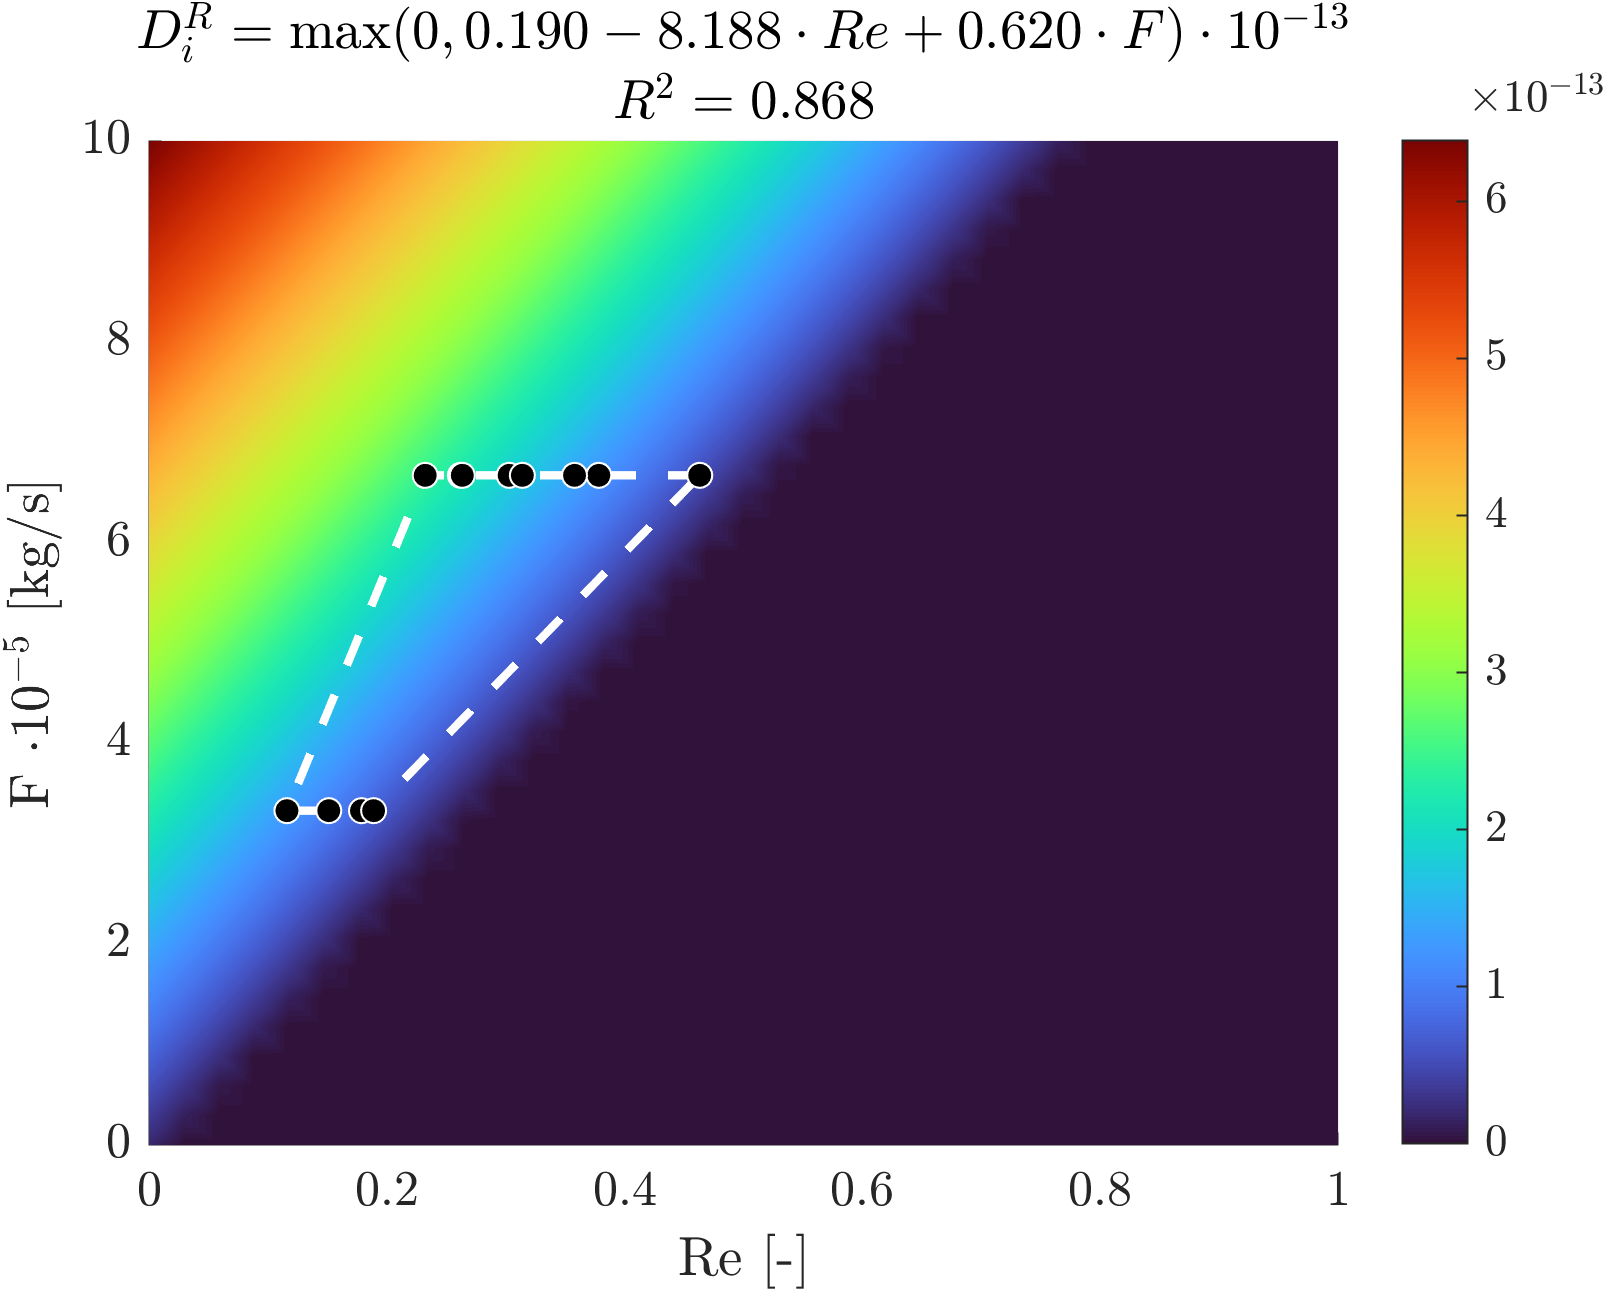
\includegraphics[trim = 0.0cm 0.0cm 0.0cm 0.0cm,clip,width=\columnwidth]{/Di.png}
		\caption{Multiple linear regression $D_i^R = f(Re, F)$}
		\label{fig:Correlation_Di}
	\end{figure}
	
	\begin{figure}[!ht]
		\centering
		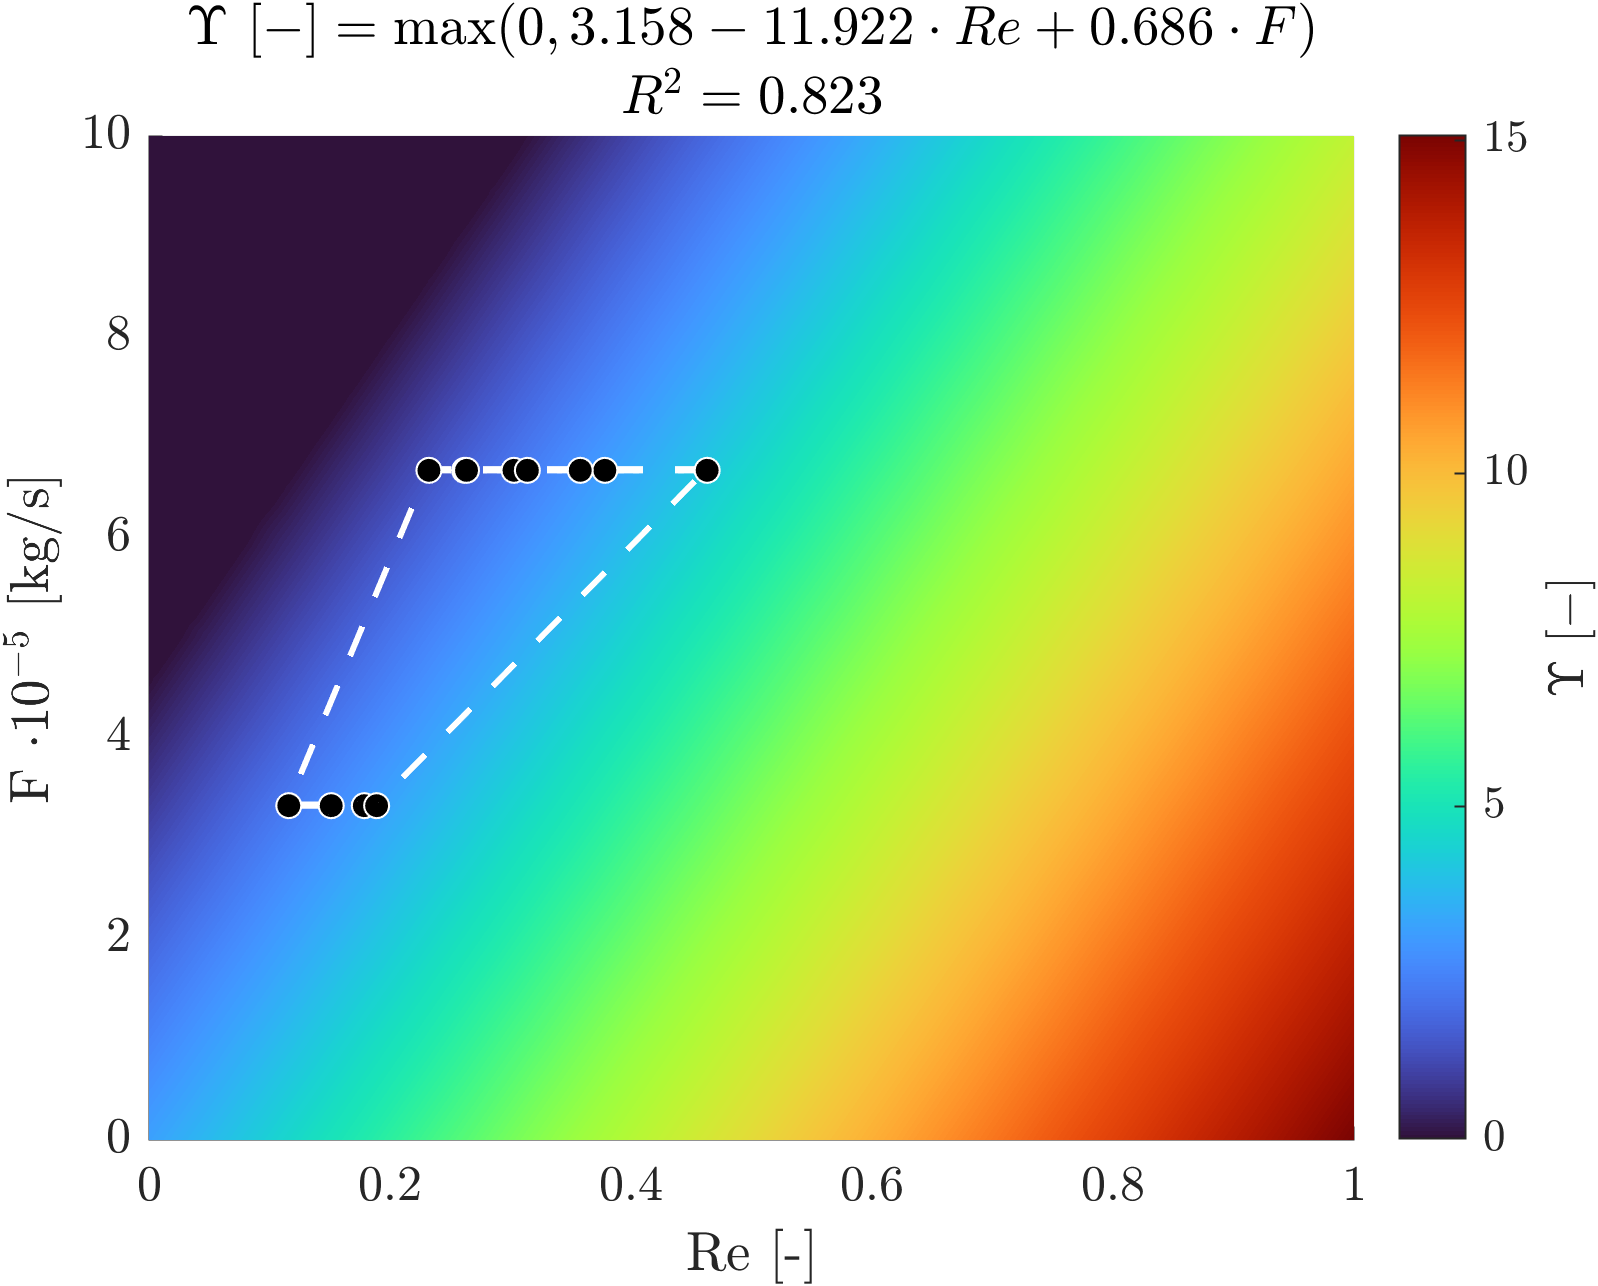
\includegraphics[trim = 0.0cm 0.0cm 0.0cm 0.0cm,clip,width=\columnwidth]{/Gamma.png}
		\caption{Multiple linear regression $\Upsilon = f(Re, F)$}
		\label{fig:Correlation_Gamma}
	\end{figure}
	
\end{document}